
    \section{Course Overview}
    \subsection{Why is Statistics Useful?}
    Physics is about reasoning about the world using our knowledge, logic, and experiments.
    Statistics is about reasoning with incomplete knowledge.
    This is a common situation for reasons we will get to later.
    Using statistics we can still make statements about certain scenarios even if we can't know something for sure.
    
    For example we will play a game.
    We have a 6 sided die (a d6) and we roll it.
    I ask you to predict the result.
    If you get it right I give you \pounds1 and if you get it wrong you give me \pounds 1.
    Is this a good bet?
    If not why not?
    We immediately know that this is a bad bet.
    If asked why we may say something like `5 times out of 6 we are going to loose and only 1 time out of 6 will we win, therefore we will lose more than we gain'.
    What if we change the amounts so instead if you are correct you get \pounds6?
    Is this now a good bet?
    It turns out it is.
    The logic is similar to before but now the possible reward has increased we actually expect to win more money than we loose even though we expect to loose more games than we win.
    Statistics and probability allow us to take scenarios like this one, and much more complicated ones, and treat them rigorously to see what we expect as an outcome.
    
    \subsection{Course Structure}
    This course is divided into 3 parts:
    \begin{enumerate}[label=\Alph*.]
        \item Basics of probability -- What is probability?
        How do we do calculations with probability?
        How do we deal with probability distributions?
        
        \item Forward logic -- Given a set up what is the probability of a given result?
        For example what is the probability that upon rolling two dice one of them gives a 6?
        What is the probability that the sum is 9?
        What is the probability that the sum is more than 5?
        
        \item Backwards logic -- Given a result what can we say about the initial set up?
        For example given results from an experiment what function can we fit to the data?
        How good is this fit?
    \end{enumerate}
    
    \subsection{Is Anything Really Random?}
    Rolling a die is a quintessential example of randomness.
    But is it truly random?
    If we know enough information about the die, for example the velocity, angular velocity, and mass of the die, as well as environmental information like the surface it is being rolled on, the viscosity of the air, etc. then in theory we could compute which face will end up on top.
    In this sense rolling dice is not \emph{truly} random.
    We say that the process of rolling dice is deterministic in that with enough information we know the outcome.
    However in practice we almost always lack the required knowledge to make this calculation so we have to treat the result of a dice roll as if it were a random event.
    
    It is also possible that not all observers have the same information.
    If I take a coin and place it in one of my hands behind my back I know where the coin is.
    The best that you can do is guess, with a \SI{50}{\percent} chance of being correct.
    In this way we see that probability is subjective in that it depends on the observer.
    
    Often all observers are in the same boat.
    Consider a mole of gas (so on the order of \(\num{e23}\) molecules).
    In principle this system is (classically) deterministic.
    Say we want to know what the velocity of a certain particle will be after some time.
    We could, in theory, start with enough information to work this out.
    However there is no practical way to do this.
    If we start with the velocity of every particle, so 3 numbers for the 3 directions, stored as 32 bit floats (the standard size for a float in C) then we have \(3\cdot 32\cdot\num{e23} = \num{e25}\) bits of information.
    That is \(\num{e9}\) petabytes.
    One petabyte of storage costs approximately half a million dollars.
    Therefore just storing the velocities of all particles costs \$500 trillion, which is about six times the world GDP.
    Clearly there is \emph{no} way that this calculation can be done by anyone.
    However we could imagine some god-like entity that \emph{could} perform this calculation so the system is still deterministic.
    It is just that the best that we can do is treat this system statistically.
    
    The final form of randomness that we will consider is \acrfull{qm}.
    In many interpretations of \acrshort{qm} there are processes that are truly random.
    For example if we have maximum information about an electron, including its spin about the \(z\)-axis, and we measure its spin about the \(x\)-axis then there is still a 50/50 chance that we measure spin up/down in that direction.
    There is no way to know before the measurement what the result will be.
    In this way \acrshort{qm} provides us with true randomness.
    However there are interpretations of \acrshort{qm} where things are deterministic and the randomness is again just missing information.
    
    We see that there are three possible levels of randomness:
    \begin{enumerate}
        \item Random for at least one observers perspective due to missing information.
        \item Random from all reasonable observers perspectives due to impracticality of computations even with perfect knowledge.
        \item Random from all observers perspectives even with perfect knowledge due to random quantum effects.
    \end{enumerate}
    All three types of randomness can be treated with statistics and probability.

    \section{Probability Basics}
    There are two ways to view probability:
    \begin{itemize}
        \item The probability of an event is the frequency with which it will occur if we are given the same starting scenario multiple times.
        This is called the frequentist approach.
        \item The probability of an event is a measure of how confident we are that that event will occur.
        This is called the Bayesian approach.
    \end{itemize}
    These two approaches are different ways of thinking but are equivalent and can be combined as long as we are careful.
    We will start by looking at the frequentist view.
    
    \subsection{Random Variables}
    To start with we will look at a random variable.
    For our purposes a sufficient definition of a random variable is a variable that has a value dependent on some random process.
    This process may be truly random or we may simply lack information required to know its value.
    Random variables can be discrete or continuous.
    It is common to use capital letters, such as \(X\), for discrete random variables and lowercase letters, such as \(x\), for continuous random variables.
    
    \subsubsection{Discrete Probability}
    Consider a discrete random variable, \(X\).
    For example \(X\) could be the value of rolling a die.
    The set \(S = \{X_i\st i\in I\}\) is called the sample space.
    It is the set of all possible outcomes, \(X_i\).
    Here \(I\) is some indexing set.
    It could be finite, such as \(I = \{1, \dotsc, 6\}\) for rolling a d6, or countably infinite, such as a process that could give any integer value where we may have \(I = \integers\).
    Starting with the same set up perform \(N\) measurements of \(X\).
    Let \(N_i\) be the number of times that we measure \(X_i\) as the value of \(X\).
    We define the probability that we measure \(X\) to be \(X_i\) to be 
    \[P_i = P(X = X_i) = P(X_i) = \lim_{N\to\infty} \frac{N_i}{N}.\]
    Here \(P_i\), \(P(X = X_i)\), and \(P(X_i)\) are just different ways to notate `the probability that we measure \(X\) to take the value \(X_i\)'.
    From the definition of \(N_i\) it is clear that
    \[\sum_{i\in I} N_i = N\]
    and therefore
    \[\sum_{i\in I} P_i = \frac{1}{N}\sum_{i\in I}N_i = \frac{N}{N} = 1.\]
    In this way we think of \(P_i\) as the normalised frequency of measuring \(X\) to have the value \(X_i\).
    
    Going back to our example of rolling a d6 we have \(S = \{1, \dotsc, 6\}\) and all probabilities are equally likely.
    Therefore we have
    \[P(X = X_i) = \frac{1}{6}.\]
    To do this calculation we used that each \(X_i\in S\) is equally likely and the total probability has to be 1.
    All being equally likely means that \(P_i = 1/|S| = 1/6\).
    We could ask a slightly more complicated question such as what is the probability that we get an even number.
    The frequentist way to answer this is to find out how many of the possible outcomes are even and collect them in a set, \(E = \{2, 4, 6\}\).
    Thus there are 3 ways to get an even number out of 6 possible results and all results are equally likely.
    Therefore
    \[P(E) = \frac{|E|}{|S|} = \frac{3}{6} = \frac{1}{2} = 0.5,\]
    which is what we would expect.
    
    We can ask a more complicated question such as what happens if we roll 2 d6?
    The sample space is now
    \[S = \{(X_i, Y_i)\st X_i, Y_i\in\{1, \dotsc, 6\}\}.\]
    We now have \(|S| = 36\).
    All possible results are still equally likely as long as we treat \((X_i, Y_i)\) as different to \((Y_i, X_i)\).
    Therefore we have \(P((X_i, Y_i)) = 1/36\) for some specific \((X_i, Y_i)\in S\).
    We now ask questions about the sum \(T((X_i, Y_i)) = X_i + Y_i\).
    For ease we list all possible values of \(X_i\) and \(Y_i\) and the sum \(T\) in table~\ref{tab:possible values of T = sum of 2 d6}.
    \begin{table}[ht]
        \centering
        \[
            \begin{array}{cc}
                & Y_i\\
                X_i &
                \begin{array}{c|cccccc}
                       & 1 & 2 & 3 & 4 & 5 & 6\\\hline
                     1 & 2 & 3 & 4 & 5 & 6 & 7\\
                     2 & 3 & 4 & 5 & 6 & 7 & 8\\
                     3 & 4 & 5 & 6 & 7 & 8 & 9\\
                     4 & 5 & 6 & 7 & 8 & 9 & 10\\
                     5 & 6 & 7 & 8 & 9 & 10 & 11\\
                     6 & 7 & 8 & 9 & 10 & 11 & 12
                \end{array}
            \end{array}
        \]
        \caption{Possible values of \(T = X_i + Y_i\) for \(X_i\) and \(Y_i\) being the result of rolling a d6.}
        \label{tab:possible values of T = sum of 2 d6}
    \end{table}
    We can treat \(T\) as a random variable.
    Say we want to know what the probability is that \(T = 5\).
    There are 36 possible pairs \((X_i, Y_i)\) and of these we see from the table that 4 of them sum to \(5\).
    Thus
    \[P(T = 5) = \frac{4}{36} = \frac{1}{9} = 0.\bar{1}.\]
    We can do this for all possible values of \(T\).
    If we do then we can list the results in another table:
    \[
        \begin{array}{c|cccccccccccccc}
            T & 0 & 1 & 2 & 3 & 4 & 5 & 6 & 7 & 8 & 9 & 10 & 11 & 12 & 13\\\hline
            N_T & 0 & 0 & 1 & 2 & 3 & 4 & 5 & 6 & 5 & 4 & 3 & 2 & 1 & 0
        \end{array}
    \]
    We can define a discrete \acrfull{pdf}, \(p\colon S_T \rightarrow [0, 1]\) where \(S_T\) is the sample space of possible values of \(T\).
    We define \(p(T_i) = P(T = T_i)\) for \(T_i \in S_T\) and \(p(T_i) = 0\) for \(T_i\notin S_T\).
    We can plot \(p\) to get a graphical representation of the various probabilities from which we can easily read off values for specific \(T_i\).
    This is what we have done in figure~\ref{fig:2d6 pdf}
    \begin{figure}[ht]
        \centering
        \includegraphics[scale=0.6]{pdf_2d6.png}
        \caption{Probability density function for the sum of two six sided dice.}
        \label{fig:2d6 pdf}
    \end{figure}
    
    \subsubsection{Continuous Probability}
    Consider a continuous random variable, \(x\).
    For example \(x\) could be the speed of a molecule in a gas.
    Again we can define a sample space \(S = \{x_i\st i\in I\}\), which is the set of all possible values for \(x\).
    Here \(I\) is an indexing set that is now uncountably infinite.
    With our example of the speed of a molecule we would expect \(S = [0, \infty)\).
    In order for probabilities to sum to 1 it is necessary that \(P(x_i) = 0\) for all \(x_i \in S\).
    Instead we can only meaningfully talk about the probability that \(x\) is in a given range.
    We define a continuous probability density function, \(p\colon S\rightarrow [0, 1]\), so that \(p(x)\dd x\) is the probability of measuring a value to be in \([x, x + \dd x]\) for some infinitesimal \(\dd x\).
    An example of a continuous \acrshort{pdf} is given in figure~\ref{fig:example continuous pdf}.
    \begin{figure}[ht]
        \centering
        \includegraphics[scale=0.6]{example_continuous_pdf.png}
        \caption{A continuous \acrshort{pdf}.}
        \label{fig:example continuous pdf}
    \end{figure}
    Using this \acrshort{pdf} we can calculate different probabilities.
    The probability of measuring \(x\) to be in \([a, b]\) is
    \[\int_a^b p(x)\,\dd x\]
    and the probability of measuring \(x\) to be greater than \(b\) is
    \[\int_b^\infty p(x)\,\dd x.\]
    This should be enough to calculate all probabilities of interest.
    
    \subsection{Calculating the Probability of \texorpdfstring{\(A\logicalAnd B\)}{A and B}}
    Independent events have no effect on each others probabilities.
    Examples of independent events are
    \begin{itemize}
        \item The values rolled on two different dice.
        \item Selecting cards with replacement.
        \item Whether it is raining and the value of the pound.
    \end{itemize}
    Dependent events are then events which do effect the outcome of each other.
    Examples of dependent events are
    \begin{itemize}
        \item Whether an integer is prime and whether that number is odd.
        \item Selecting cards without replacement.
        \item Whether it is raining and the number of umbrellas in use.
    \end{itemize}
    
    Let \(A\) and \(B\) be two different events.
    We wish to know the probability that both \(A\) and \(B\) occur.
    We denote this \(P(A\logicalAnd B)\) or \(P(A, B)\).
    Viewing \(A\) and \(B\) as sets of possible outcomes we may also write it as \(A\intersection B\).
    Viewing \(A\) and \(B\) as hypotheses (as we will do later) we may write it as \(A\conjunction B\).
    We will start with an example.
    
    Take the following 6 cards from a deck: \(J\diamondsuit\), \(Q\diamondsuit\), \(K\diamondsuit\), \(J\clubsuit\), \(Q\clubsuit\), and \(K\clubsuit\).
    Separate the cards into the two suits and shuffle each triplet of cards.
    From each triplet select one card.
    What is the probability of getting 2 kings?
    First note that the two cards we get are independent events.
    The possible pairs are best described in the following table, with the number of kings in the pair listed:
    \[
        \begin{array}{c|ccc}
            & J\clubsuit & Q\clubsuit & K\clubsuit\\\hline
            J\diamondsuit & 0 & 0 & 1\\
            Q\diamondsuit & 0 & 0 & 1\\
            K\diamondsuit & 1 & 1 & 2
        \end{array}
    \]
    We see that there are 9 possible pairs \((X\diamondsuit, Y\clubsuit)\) where \(X, Y\in \{J, Q, K\}\).
    Of these only one pair has two kings, \((K\diamondsuit, K\clubsuit)\).
    Therefore the probability of getting two kings is
    \[P(\text{2 kings}) = P(K\diamondsuit \logicalAnd K\clubsuit) = \frac{1}{9} = 0.\bar{1}.\]
    Note that this is the same as
    \[P(K\diamondsuit)P(K\clubsuit) = \frac{1}{3}\cdot\frac{1}{3} = \frac{1}{9} = 0.\bar{1}.\]
    What if instead we shuffled all 6 cards together and then picked two cards without replacement?
    The first time we pick a card there are 6 cards and 2 of them are kings so the probability that we get a king is
    \[P(\text{first card is a king}) = \frac{2}{6} = \frac{1}{3} = 0.\bar{3}.\]
    The second time we pick a card there are 5 cards but the number of kings depends on what we picked the first time.
    Since we want two kings we assume that the first time we picked a king (if we didn't there would be no way to get 2 kings).
    Therefore there is 1 king left.
    We then calculate the probability of selecting a king given we have already picked a king.
    In general the probability of event \(B\) given that event \(A\) has occurred is \(P(B|A)\).
    The probability that we get a king the second time given we got a king the first time is
    \[P(\text{second card is a king}|\text{first card is a king}) = \frac{1}{5} = 0.2.\]
    We can now calculate the probability that we select two kings:
    \[P(\text{2 kings}) = P(\text{first card is a king})P(\text{second card is a king}|\text{first card is a king}) = \frac{1}{3}\cdot\frac{1}{5} = \frac{1}{15} = 0.0\bar{6}.\]
    
    In general we find that for two events \(A\) and \(B\) the probability that both occur is
    \[P(A\logicalAnd B) = P(A)P(B|A).\]
    Note that if \(A\) and \(B\) are independent then \(B\) is equally likely to occur whether or not \(A\) occurs so \(P(B|A)\) reduces to \(P(B)\).
    Therefore this formula works regardless of whether \(A\) and \(B\) are independent.
    
    We can view \(A\) and \(B\) as sets of possible outcomes.
    In this case
    \[P(A) = \frac{|A|}{|S|},\qquad\text{and}\qquad P(B) = \frac{|B|}{|S|}\]
    where \(S\) is the sample space.
    We can view the possible outcomes visually in figure~\ref{fig:venn diagram for events A and B}.
    \begin{figure}[ht]
        \centering
        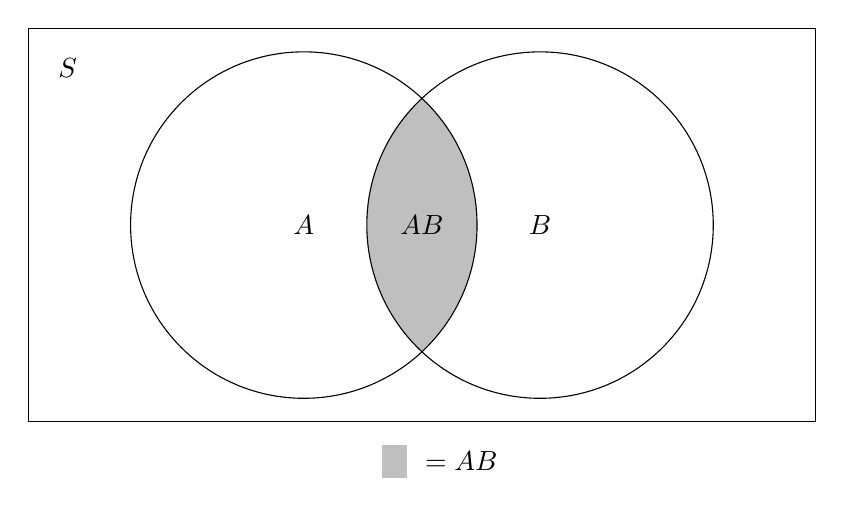
\begin{tikzpicture}
            \draw (0, 0) rectangle (10, 5);
            \node at (0.5, 4.5) {\(S\)};
            \begin{scope}
                \clip (3.5, 2.5) circle[radius=2.2cm];
                \clip (6.5, 2.5) circle[radius=2.2cm];
                \draw[fill=lightgray] (0, 0) rectangle (10, 5);
            \end{scope}
            \draw (3.5, 2.5) circle[radius=2.2cm];
            \draw (6.5, 2.5) circle[radius=2.2cm];
            \node at (3.5, 2.5) {\(A\)};
            \node at (6.5, 2.5) {\(B\)};
            \node at (5, 2.5) {\(A\intersection B\)};
            \node at (5.5, -0.5) {\( = A\intersection B\)};
            \draw[fill=lightgray, color=lightgray] (4.5, -0.7) rectangle (4.8, -0.3);
        \end{tikzpicture}
        \caption{Venn diagram for events \(A\) and \(B\)}
        \label{fig:venn diagram for events A and B}
    \end{figure}
    In this figure the shaded area represents the outcomes that are in \(A\) and \(B\), this is the intersection, \(A\intersection B\), of the sets \(A\) and \(B\).
    Like any probability viewed as sets we calculate the probability as
    \[P(A\logicalAnd B) = P(A\intersection B) = \frac{|A\intersection B|}{|S|}.\]
    
    Note that `\(\logicalAnd\)' is symmetric.
    That is \(P(A\logicalAnd B) = P(B\logicalAnd A)\).
    This means that
    \[P(A\logicalAnd B) = P(A)P(B|A) = P(B)P(A|B) = P(B\logicalAnd A).\]
    Rearranging this we get
    \[P(B|A) = \frac{P(A|B)P(B)}{P(A)}.\]
    This is known as Bayes' theorem and it turns out to be very important in Bayesian statistics.
    
    \subsection{Calculating the Probability of \texorpdfstring{\(A \logicalOr B\)}{A or B}}
    Mutually exclusive events cannot both occur at the same time.
    For example getting heads and tails are mutually exclusive.
    On the other hand a number being even and a prime is possible so even and prime are not mutually exclusive.
    If two events, \(A\) and \(B\), are mutually exclusive then \(P(A\logicalAnd B) = 0\), or in terms of sets \(A\intersection B = \emptyset\).
    We can represent mutually exclusive events graphically, as we have in figure~\ref{fig:mutually exclusive events}.
    We see that \(A\intersection B = \emptyset\) so \(|A\intersection B| = 0\).
    Since there is no overlap between the two sets the size of the union is the sum of the size of the two sets:
    \[|A\union B| = |A| + |B|.\]
    Therefore the probability of \(A \logicalOr B\) is
    \[P(A\logicalOr B) = \frac{|A| + |B|}{|S|} = P(A) + P(B).\]
    \begin{figure}[ht]
        \centering
        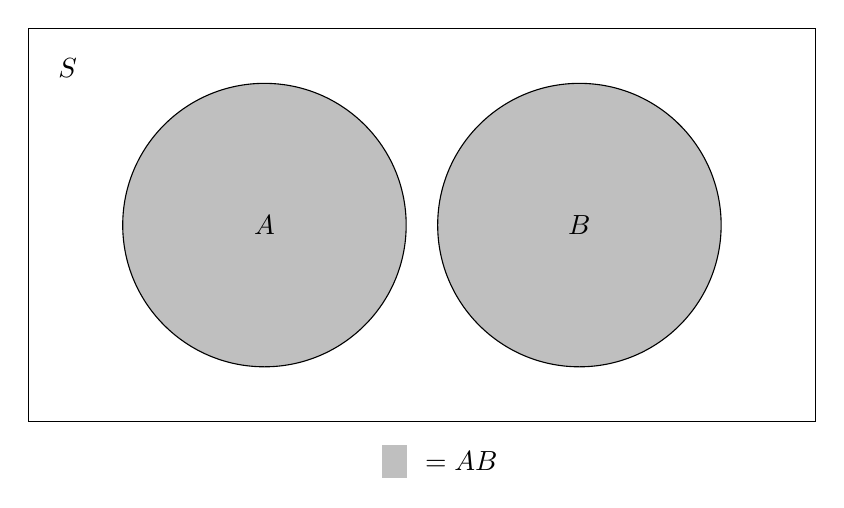
\begin{tikzpicture}
            \draw (0, 0) rectangle (10, 5);
            \node at (0.5, 4.5) {\(S\)};
            \begin{scope}
                \clip (3, 2.5) circle[radius=1.8cm];
                \draw[fill=lightgray] (0, 0) rectangle (10, 5);
            \end{scope}
            \begin{scope}
                \clip (7, 2.5) circle[radius=1.8cm];
                \draw[fill=lightgray] (0, 0) rectangle (10, 5);
            \end{scope}
            \draw (3, 2.5) circle[radius=1.8cm];
            \draw (7, 2.5) circle[radius=1.8cm];
            \node at (3, 2.5) {\(A\)};
            \node at (7, 2.5) {\(B\)};
            \node at (5.5, -0.5) {\( = A\union B\)};
            \draw[fill=lightgray, color=lightgray] (4.5, -0.7) rectangle (4.8, -0.3);
        \end{tikzpicture}
        \caption{Mutually exclusive events}
        \label{fig:mutually exclusive events}
    \end{figure}
    If instead we take \(A\) and \(B\) to not be mutually exclusive then we have a scenario more like figure~\ref{fig:not mutually exclusive events}.
    In this case we have \(A\intersection B \ne \emptyset\) so \(|A\intersection B| \ne 0\).
    Note that we say \(A\) and \(B\) are disjoint sets if \(A\intersection B = \emptyset\).
    We need to find \(|A\union B|\).
    We start with the naive answer of \(|A\union B| = |A| + |B|\) but we notice that this isn't quite right.
    Say \(x\in A\intersection B\) then \(x\) is counted in \(|A|\) and \(|B|\).
    We therefore count everything in \(A\intersection B\) twice.
    To remedy this we subtract the size of the intersection to get
    \[|A\union B| = |A| + |B| - |A\intersection B|.\]
    \begin{figure}[ht]
        \centering
        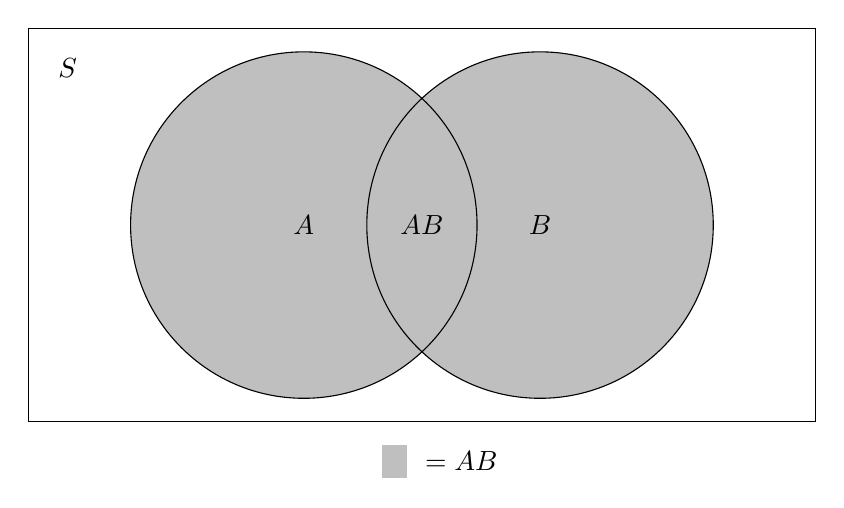
\begin{tikzpicture}
            \draw (0, 0) rectangle (10, 5);
            \node at (0.5, 4.5) {\(S\)};
            \begin{scope}
                \clip (3.5, 2.5) circle[radius=2.2cm];
                \draw[fill=lightgray] (0, 0) rectangle (10, 5);
            \end{scope}
            \begin{scope}
                \clip (6.5, 2.5) circle[radius=2.2cm];
                \draw[fill=lightgray] (0, 0) rectangle (10, 5);
            \end{scope}
            \draw (3.5, 2.5) circle[radius=2.2cm];
            \draw (6.5, 2.5) circle[radius=2.2cm];
            \node at (3.5, 2.5) {\(A\)};
            \node at (6.5, 2.5) {\(B\)};
            \node at (5, 2.5) {\(A\intersection B\)};
            \node at (5.5, -0.5) {\( = A\union B\)};
            \draw[fill=lightgray, color=lightgray] (4.5, -0.7) rectangle (4.8, -0.3);
        \end{tikzpicture}
        \caption{Not mutually exclusive events}
        \label{fig:not mutually exclusive events}
    \end{figure}
    This formula actually also works if \(A\) and \(B\) are disjoint as then \(A\intersection B = \emptyset\) so the final term is zero.
    Therefore this formula works regardless of whether or not \(A\) and \(B\) are mutually exclusive.
    The probability that event \(A\) or \(B\) or both occur is
    \[P(A\logicalOr B) = P(A\union B) = \frac{|A| + |B| - |A\intersection B|}{|S|} = P(A) + P(B) - P(A\logicalAnd B).\]
    
    \subsection{Probability as Degree of Belief}
    So far we have used a frequentist approach to probability.
    A Bayesian approach involves hypotheses.
    A hypothesis is a statement, \(H\), that is either true or false.
    We can assign to each hypothesis a number, \(C(H)\), representing its credibility.
    Let \(S = \{H_i\st i\in I\}\), where \(I\) is some indexing set that will be countable if \(H_i\) involves discrete variables, or uncountable if \(H_i\) involve continuous variables. \(S\) is the sample space, that is the set of all possible hypotheses. \(C\colon S \rightarrow [0, 1]\) is defined so that \(C(H)\) is the credibility of \(H\).
    It can be shown that there is a unique way to assign a credibility to  \(H_i\) if we require the following to hold:
    \begin{enumerate}
        \item \(C(H_1) > C(H_2)\) if we have a stronger belief in \(H_1\) than \(H_2\).
        \item \(\sum_i H_i = 1\).
        \item \(C(H_1\conjunction H_2) = C(H_1)C(H_2|H_1)\) where \(\conjunction\) represents the Boolean operator and.
        \item \(C(H_1\disjunction H_2) = C(H_1) + C(H_2) - C(H_1\conjunction H_2)\) where \(\disjunction\) represents the Boolean operator or.
    \end{enumerate}
    If we take these rules and identify \(C \leftrightarrow P\) and \(\conjunction/\disjunction\leftrightarrow \intersection/\union \leftrightarrow \text{and}/\text{or}\) then we recover the frequentist results.